\documentclass{article}
\usepackage{color}
\usepackage{pdfpages}
\usepackage{ifthen}
\newcommand{\showColour}{yes} % {yes}
\newcommand{\showComments}{yes} % {yes}
\newcommand{\note}[2]{\ifthenelse{\equal{\showColour}{yes}}{\textcolor{#1}{#2}}{#2}}
\newcommand{\jwb}[1]{\note{blue}{#1}}

\newcommand{\paolo}[1]{\note{magenta}{#1}}


\newcommand{\com}[2]{\ifthenelse{\equal{\showComments}{yes}}{\textcolor{#1}{#2}}{}}
\newcommand{\comment}[1]{\com{red}{#1}}


\begin{document}


Dear Dr. Bryans,

Thank you for submitting your manuscript to Future Generation Computer Systems. I have received comments from reviewers on your manuscript. Your paper should become acceptable for publication pending suitable minor revision and modification of the article in light of the appended reviewer comments.

When resubmitting your manuscript, please carefully consider all issues mentioned in the reviewers' comments, outline every change made point by point, and provide suitable rebuttals for any comments not addressed.


\section*{Comments from the editors and reviewers:}
\section*{Reviewer 1}

The authors have addressed the concerns, but have indeed raised some others:

\begin{enumerate}
\item The authors use the following words interchangeably: abstraction, obfuscation, and hiding of information. These terms are not similar, and have been used carelessly in the title and the Introduction. For review:

* Obfuscation is typically applied to programs to make it "harder to understand". Christian Collberg, Clark Thomborson, and Douglas Low. A taxonomy of obfuscating transformations. Technical Report 148, Department of Computer Science, University of Auckland, July 1997.

* Abstraction is to provide a conceptual view, typically of data structures.  "An abstraction denotes the essential characteristics of an object that distinguish it from all other kinds of object and thus provide crisply defined conceptual boundaries, relative to the perspective of the viewer."

* Hiding of information is similar to encapsulation. From OO design:"The process of hiding all the details of an object that do not contribute to its essential characteristics; typically, the structure of an object is hidden, as well as the implementation of its methods. The terms information hiding and encapsulation are usually interchangeable."


From OO design the correct term in this work to use is encapsulation and not obfuscation or abstraction.

A consequence of this verbiage are the title (Abstracting PROV...) which and the incorrect sentence such as following: "As we will see in the rest of the paper, replacing the three selected nodes with a single abstract node (an activity in this case) while preserving the validity of the document, requires that all other nodes that lie on the directed paths that connect these nodes are also removed." The nodes are technically not removed but hidden or encapsulated. 

It is strongly recommended that authors review the draft from the perspective of these definitions. 


\jwb{Change abstraction $->$ encapsulation throughout. It should be easy enough. The reviewer clearly feels strongly about it. JWB to do.}

\jwb{Remove Fig. 6 (the example of what goes wrong) and go directly into the solution we propose. JWB to do.}

\jwb{Rebuild figures. JWB to do.}

\jwb{Para on trust model. PM to do}

\item The introduction does not mention anything about the trust model between PA and IP on obtained provenance. Specifically if PA does not trust the obtained report, what guarantee does it have for trusting the obtained provenance. The authors must provide explanation as to why they think provided provenance will be trusted by PA. 

 \jwb{A paragraph on the trust model will help. Limited trust (hence I don't show you everything), but a willingness/need to cooperate. (hence I show you something) Illustrate with disaster relief/military applications.  PM to do.}

\item Related Work


1. There are many differences that this work has with Zoom, but to assert that in Zoom the user requires knowledge about the underlying graph topology is incorrect. In Zoom user knows the relevant modules (which are resented as nodes) and chooses  amongst the internal nodes to display—it does not substitute the entire subgraph with another abstract node.  A view is typically to improve readability of large graphs—and that is the notion used in Zoom, but is different than an encapsulation which is specifically for hiding information. Thus, Zoom does not prevent a reader to expand the view and see the original graph, but the  system being proposed in the article will never divulge underlying information. 


2. There is confusion when the actions are user-defined and when dictated by the underlying topology. In comparing Zoom the authors state “In Zoom, the user is aware of underlying topology and and in their case the user need not be”. In comparing [19], they say “the aggregation operator is entirely driven by graph topology and not by a user choice”. The latter sentence by inference implies that their approach is driven by user choice, and since any form of aggregation/grouping requires knowledge of graph topology, by consequence, the user is aware of the topology. This conflicts with their statement contrasting Zoom.


The above sentence must be made more specific. 
\jwb{make sentence more specific! PM to do.}

\item The paper introduces three operators: path closure, extend, and replace, and provides either a extension and replace or just closure and replace. It is not clear when the IP or the system will chose one operator over the other. The time complexity appears to be the same. So why will extend and replace ever be applied over path closure and replace?

  \jwb{It isn't a choice. I wonder if Fig 6 gives that impression?}
  

\item There are several issues with Fig 6. 

  \begin{enumerate}
    
\item The basis for the position of e’ in Fig 6 is not clear. Why in between a1, a3 and a2, a4? Why not, for instance, as a substitute for e1? If this choice of representation is one chosen by authors, then it should be mentioned. 


  \jwb{Fig 6. is an example of what goes wrong. A couple of reviewers have had a problem with this (or the same one twice). We should either remove it or flag very carefully that it is a strawman.}

\item In group, the authors use the term “rewired” but do not explain what that means. If rewired means ALL incoming and outgoing edges are connected back again, then what happened to edge a1->e1 and a3->e3? The explanations are confusing: it seems the direction of the edge is introduced but this edge is also relabeled ‘wgBy’. Why? 

\jwb{he's right about this. It should be labelled wgBy and used. }
  
It might be helpful in that Figure to show how each edge in the left hand side of the diagram is mapped to each edge in the right hand side of the diagram.  

\jwb{I think the reviewers are overthinking this example.}

 The definition of Group operator is a node grouping operator; the definition does not include edges. But group operator is stated as an alternative to path closure, replace, extend.

\jwb{The reviewer is wrong here. 'Group' returns a PROV graph. Group is defined using path closure, replace and extend. The rewiring is part of the definition, defined in replace.}
 
Why are edges a1->e1 and a->e3 not left unlabeled because ‘used’ edge label will lead to a false dependency. Again the group operator definition does not imply a false dependency may result as a result of it. 

\jwb{Again, the reviewer is reading this not as an example of what goes wrong, but of our contribution. }

\item There is something wrong with the mathematical definition: $PG_{gu/ea}  ~~X~~ P(V) \rightarrow PG_{gu/ea}$

  
 The result is the same graph?  As a side, the equations are not numbered, and P(V) in this equation is not defined.

 \jwb{This is not a definition, it's the type of the Group operator. (Page 14) Say this explicitly. }
 \jwb{Overall, I recommend removing fig 6 and the paras beginning ``to get a quick intuition''. Replace with a para on the functional approach then  go into the definition of path closure.}

\item The definition of Group operator is a node grouping operator; the definition does not include edges.

\jwb{No, the definition is in terms of extend, closure and replace. The edges are dealt with by the replace operator.}

  
\item Explain why these cycles cannot be broken by simply keeping timing information or “happens before” relationship. 

\jwb{I'm not sure what this means, or what the reviewer is referring to}
  
  \end{enumerate}

\item refers to “issue”. Which one? Previous para states two issues. 

  \jwb{This is referring to the para before section 4.1. Both problems are caused by the nodes $a_1$ and $a_3$.
    }
 \jwb{This is another example of Fig 6 being a problem (at least for this reviewer)}


\item it is not clear why the type of $v_d$ and $v_s$ are necessary in definition when G is an element of $PG_{gu/ea}$.

\jwb{t is the type of the nodes on the boundary that Extend creates. Add sentence under definition of extend (defintion 3) JWB to do.}

\item Figure 8 uses a new keyword ’absorb’. Why isn’t it ‘extend’ now?

\jwb{Historical reasons! JWB to fix.}   

\item How is Definition 6 related to the grouping operator? Is it related?

The significance of this definition is not clear. 

  \jwb{Let's remove defn 6. JWB to do.}

\item In Section 4.2 the word propagation is used. Is it similar to extension? 

  \jwb{Similar. Perhaps avoid the word.  I think the first reviewer just gave up here. JWB to correct.} 

  
\end{enumerate}

\subsection*{Reviewer 2}

   \subsubsection*{Summary}

This paper is about abstracting provenance graphs, using the PROV model promulgated by the W3C.  PROV graphs include nodes that can be entities, activities or agents, and edge relationships indicating usage, generation, invalidation, association, attribution, delegation, and other relationships between them.  Given such a graph, describing a history or trace of a process, a common concern is to hide information according to some policy.  Provenance abstraction is a subproblem arising when we have identified a set of nodes we wish to abstract (i.e. collapse into a single node).  This paper considers the problem: if the input graph is a "valid" one according to the PROV standard (specifically, the validity constraints in the PROV-CONSTRAINTS standard), what other nodes/edges need to be collapsed, or other changes to the graph made, so that the result is still valid?  There are several difficulties: collapsing nodes of different types into a single node (of a given type) may result in edge relationships needing to be adjusted,  additional nodes may also need to be collapsed in order to avoid cycles, etc.

The paper first considers the subcase where there are only two node types (entity/activity) and two edge relationships (usage/generation). Thus, the graph is bipartite.  Formal definitions of the problem and proposed algorithm are given: first the set of nodes is closed-off to include all nodes "between" selected nodes, then additional nodes on the frontier of the selected set are added so that the outside of the selected set matches the intended collapsed node type.  The paper considers the constraints and argues that abstracting a valid graph results in another valid graph.  Next the paper shows how to extend the results to consider PROV graphs with agents, with an unstated assumption that agent nodes are disjoint from entity and activity nodes, so that the agent nodes only interact with the rest of the graph in fairly limited ways and the underlying bipartite abstraction approach still works.

\jwb{is this assumption not always true? PM to clarify.}

One complication in this setting is that edges from agents to abstracted nodes may no longer make sense, and in this case they are removed.

\subsubsection*{Evaluation}

The problem being considered seems challenging and I think a good solution would be worthy of publication.  However, I'm not yet persuaded that the approach presented in the paper is sufficiently motivated and justified.  

\begin{enumerate}
\item The problem seems under-specified.  The abstract states two goals for abstraction: first, the abstract version of the document should be valid if the original version is, and second, the dependencies (edges) in the abstract version should be justified by those in the original.  (Section 1.2 and the conclusion likewise asserts that abstraction will not introduce false information, but I don't see where this is actually proved.) However, the second goal is not captured formally, and I think there is a third important goal that is not mentioned at all: that the abstracted document should not "abstract away too much".

  
For example, one (unserious) solution could be to abstract the whole graph to a single node, discarding all edges.  This would be correct (the internal details of the abstracted subgraph are definitely hidden, all right) but is not "optimal" in some sense among the correct solutions.  Another slightly less silly solution could be to discard the entire abstracted set (and all incident edges), resulting in a PROV graph that is still valid, hides the intended information, but still abstracts "too much" in some sense since there is nothing represented the abstracted nodes.  What is missing to rule out both silly solutions] is some condition that says you can't throw "too much" of the PROV graph away, for example, saying that parts of the graph that have nothing to do with (i.e. not neighbors of) an abstracted node should not be affected.  



\begin{figure}
  \centering
  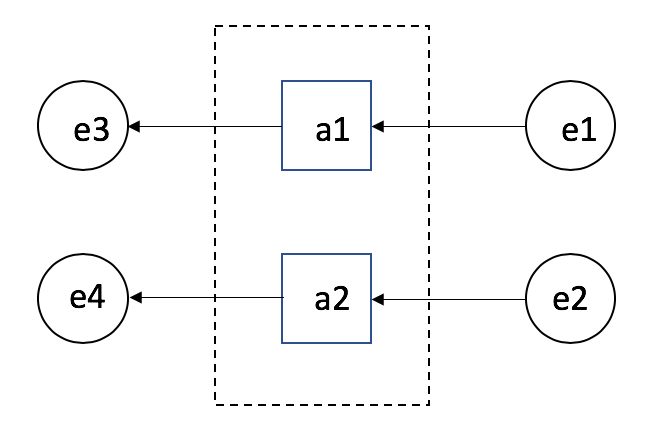
\includegraphics[scale=0.3]{example1.png}
  \caption{  \label{fig:example1} no false dependencies}
\end{figure}

\jwb{We are rather vague about ``no false dependencies''. For example in the figure~\ref{fig:example1}, the abstraction introduces an apparent dependency between e1 and e4 that was not there previously.  I suggest we ``refine the assumption'' to be ``no unjustified dependencies'' where a dependency is justified if it is made of relationships all of which are justified and a relationship is justified if it was present in the original graph. The problem then reduces to showing that we introduce no unjustified links in the group operator, which we can do by inspection of replace. JWB to do. }
  
In addition, I think the notion of correctness of abstractions in this paper needs to be compared with the notion of "sound" workflow views explored for ZOOM by Liu et al. [A].


\item I did not really follow the discussion of preservation of constraints in section 5.  I consider myself fairly familiar with the constraints specification.  The specification (and the accompanying semantics) does not assume the events are linearly ordered, and the authors correctly point this out.  However, the argument that the constraints are satisfied by the abstracted document seems to hinge on being able to compute maxima and minima among (finite) sets of events.  This may not be possible in a general preorder, so using the notation for "max" and "min" is not necessarily meaningful, since the max or min of a set may not exist. As a simple example, suppose we have two parallel chains e1 wgb a1 used e2 and e3 wgb a2 used e4.  Then the events related to e1/a1/e2 are unrelated to those for e3/a2/e4, for example the max and min of the two concurrent usage events doesn't exist.

  \jwb{This is Figure~\ref{fig:example1}, but I don't follow the argument. max and min of finite sets exist. PM to deal with. }

Another (more minor but relevant) nitpick is that the ordering in a PROV graph is a preorder (aka quasiorder), so that there can be nontrivial cycles in the $\leq$ relation (for example for "simultaneous" generation events).  This means that if an upper bound or lower bound exists for a set of events, it may not be unique.
This also seems likely to lead to strange situations, for example if abstraction leads to two generation events becoming simultaneous, it will seem strange if they have different timestamps (though there is nothing wrong with this vis a vis validity since the timestamps are just uninterpreted data as far as PROV validity is concerned.)  Yet in several places the paper assumes that simultaneous events are necessarily equal, which is not the case in PROV.

\jwb{I'm lost here too. PM to deal with.}

I think this difficulty can be overcome by, for example, assuming that you are given an event preorder consistent with the original PROV instance and constructing from that another preorder consistent with the abstracted instance in which the needed maximal or minimal events exist, adding them if necessary, and choosing the maximum or minimum of a set of events arbitrarily if there is more than one possibility.  



\item It is fine and reasonable that the paper mostly focuses on the entity/activity/generation/use subset of PROV.  The later section on extending to include agents, however, implicitly relies on some simplifying assumptions.  In PROV, entity and activity are disjoint classes, but agent is not assumed to be disjoint from either entity or activity.  So, a node could be both entity and agent, or both entity and activity (just not entity and activity or all three).  I think this possibility would lead to some complications compared to the simple case discussed in the paper, and this simplifying assumption (that agents, entities and activities are disjoint) should be made explicit.

\jwb{Yes, it certainly would! And we do make the implicit assumption that agents are disjoint from entities and activities. Soln: just say so somewhere. JWB to do.}
  
Another related point is that by assuming that nodes/edges have exactly one PROV type, the paper may miss an opportunity for using flexibility that already exists in PROV to aid abstraction.  For example, nothing in PROV says that a node has to have any type at all; and though edges are expected to have a property type, PROV provides a generic edge type "wasInfluencedBy" that superclasses the other edge types.  Thus, the problem with edges becoming isolated discussed in section 6.3 could be avoided by using wasInfluencedBy edges to represent the problematic edge relationships, instead of deleting such edges and removing the resulting disconnected nodes.  Alternatively, the issue highlighted in figure 15 could be avoided by instead allowing eN to be both entity and agent, so that the actedOnBehalfOf edge still makes sense.  (However, I'm not sure this works in general and would result in graphs that no longer have agents distinct from entity /activity nodes.)

\jwb{Best just say this isn't a direction we go in. Just say that graphs are bi-partite. JWB to do. } 

\item A relatively minor point is that there is some further uncited work on provenance sanitization/abstraction/redaction [A,B,C,D].  The notion of convexity mentioned here appears also in [B] for example, which only considers activity abstraction for a simplified form of OPM.  There is also a short survey [E] which already discusses/compares work up to circa 2014.

\jwb{Only A and B are mentioned below. Maybe we could track the others down, or ask the editor for clarification? PM to do a lit survey. } 
\end{enumerate}


Overall, I think the paper presents work that is worth publishing: I started out thinking the problem and solution seemed a bit simplistic, but the more I thought about (and read) the paper the more I realized that there are some nontrivial subtleties.  However, the above issues need to be addressed.  Given that I've been asked to review this after one round of reviewing and revision has already been performed, I hesitate to require major revision, so instead I'll suggest the following changes that could be made in a minor revision round:

\begin{enumerate}

\item Clarify what part of the paper proves that that relations in the abstracted graph are "justified", and discuss the issue of how to avoid "abstracting too much".

\jwb{I think we can answer this, as I suggest in answer to Point 1. JWB to do.}

\item Clarify the discussion of max/min and avoid apparent reliance on the maxima/minima already existing in the event structure for the original document.

  \jwb{Dont' know here PM to do.}

  
\item Clarify assumptions needed for the existing algorithm to work in the presence of agents.

\jwb{OK - mainly that the node types are disjoint JWB to do.}
  
\item Discuss alternative abstraction strategies such as using wasInfluencedBy edges.

  \jwb{A brief discussion with a point forward to Blue/Collapse paper? I've forgotten how we agreed to deal with this.}
  
\item Cite/discuss uncited related work and compare with other formal notions of abstraction correctness such as "sound workflow views"

 \jwb{perhaps do a search for these. PM to do lit survey.}
  
\end{enumerate}

These changes would help to circumscribe the contribution of the paper more clearly, and identify possible areas for further work building on it.

Of course, I would also be happy with more substantial changes that address the concerns above more thoroughly.

\subsubsection*{Detailed comments}

\jwb{Mostly, I can do these.}

The paper is overall in fairly good shape, there were few typos or difficult-to-follow points.

p10: "Further extensions... wasDerivedFrom and wasInformedBy" - while wasInformedBy in Prov is just an abbreviation for a 2-step generation/use path, wasDerivedFrom is a little more complicated (it can correspond to a chain of use/generation steps) and has a special status in PROV-CONSTRAINTS: it is the only relationship where event ordering cycles are strictly forbidden.  Incidentally, this means that in the absence of wasDerivedFrom, it's easy in some sense for a document to be valid, as long as it is well-formed, all of the events can be simultaneous.  
\jwb{Not sure what to do about this one. What are we being asked to do? Still not sure here.}


p12.  I think it would help discussion to clarify that there might be many preorders $(Ev,\preceq)$ that are consistent with a given, valid PROV document, and throughout this and the next section you are fixing one such preorder.  I think it would also be helpful (if you do as I suggest above) to distinguish between the preorder $(Ev,\preceq)$ that is given for the original document, and a new one that you construct $(Ev',\preceq')$, that extends $(Ev,\preceq)$ with any new events needed to describe the new edge relationships introduced for the abstracted node.  Likewise, it would be helpful to state the constraint-preservation result somewhere explicitly as a theorem so that it is clear what formal property corresponds to the informal description given earlier.

\jwb{OK, I think I see this one. I guess the theorem he talks about is the one proved in the two appendicies.}


p12.  In the formula $\preceq \subset Ex \times Ev$, there should be space between the preorder and subset symbols

p12.  Missing colon/punctuation after "in [9])"

p13, In C7, I think the RHS should be end(a), not ev(a).

p13, in C8, you say that two invalidation events for the same activity are equal, but (as for C2)they need not be equal, just simultaneous.

p15 "subgraph given by pclos" - since pclos returns a set of nodes, not a graph, did you mean to say "subgraph induced by pclos"?

p16.  The figures fall off the edge of the page.

p17.  In definition 3 and following discussion, I had to think for a minute to convince myself that extend correctly ensures that boundary nodes are of type t.  I think this happens to be the case for bipartite $PG_{gu/ea}$ graphs.  The definition ensures that all added nodes are of type t, but if more edges or node types are present then it seems possible that this definition might leave some boundary nodes of other types. \jwb{It's because we are assuming here that $t\in\{e,a\}$  } Please say a little more here since this fact is relied on later and then when agents are considered I think the correctness of extend when t = e or a needs to be revisited. \jwb{Need to think about this point}

p21.  In the "if $|V_{gen}| \leq 1$" side condition, there is unnecessary spacing between "|" and "V" and missing spacing between "|" and "$\leq$".

p21. "v2 is reachable from v2" - I think one of these was meant to be v1.

p22. "And secondly, in a provenance graph ... the graph is bipartite" - true for $PG_{gu/eq}$ but not generally.  Also, "with respect of" -> "with respect to" 

p22. "the theoretical max" -> "... maximum"

p22. "will have to hidden" - missing "be"

p23. In section 5 it is implied that we can reason about ordering constraints (i.e. a preorder) by reasoning about all the possible linear orderings consistent with the preorder, and perhaps this is the rationale for using min and max.  However, I am not sure that introducing discussion of linear orderings is necessary or helpful here; I think it would be clearer to present the content of this section as a recipe for constructing an event preorder for the abstracted graph G' from any such preorder consistent with the original graph G, adding any necessary min/max events.

\jwb{Paolo - would this be a helpful way to look at it?}

p24. In figure 10, I was uncertain whether your model allows multiple edges of the same kind between two nodes.  The formal definition of the model doesn't appear to allow this; PROV does, but does so by assigning identifiers to use/generation/etc relations, which are not modeled explicitly here.  (but then on page 24 you say you are going to use such identifiers for convenience anyway).



p24. "wgby" was elsewhere called genBy as well as wgBy (in figures)

p27 "Let V* to" - remove "to"

p27.  "abstracted prov graph" -> "...PROV..."

p27.  "following equalities, define" remove comma

p28. Most of the definitions in this section have "e-grouping" in parentheses except definition 11.  This seems inconsistent (though I think you could get rid of all of them).  Also, why isn't definition 11 exactly like definition 9 up to symmetry?

\jwb{Don't know..}

p30.  In definition 15, the generation events are simultaneous but not necessarily equal. 

p30. "the event of the invalidation event" - there seem to be extra words

p34: "agent nodes are always the targets of directed edges" - this relies on the unstated assumption that agent nodes are disjoint from entity/activity nodes.  In general, an agent node that is also an entity or activity could be the source of a directed edge (use, generation etc.)

\jwb{must make this assumption clear}

p34. "or its symmetric," -> "or its symmetric form,"

p35.  There are occurrences of both "obo" and "abo" as abbreviations for "actedOnBehalfOf", please make consistent.



p36.  Removing edges and removing isolated nodes seems undesirably lossy to me.   For example if there was already an isolated agent node in the graph you would discard it even though it was not disconnected as a result of abstraction.
\jwb{good point}
Edges that are no longer well-typed could be replaced with wasInfluencedBy edges which can link any entity/activity/agent nodes.  This would avoid the disconnection problem.
Anyway, if you solve the disconnection problem by discarding isolated nodes, you might still wind up with a less connected graph (e.g. what if ag4 in figure 15 was also acting on behalf of some ag5). These won't be discarded because they are not isolated.
\jwb{not sure how to solve this one}

p37. "will not introduce false information" - as mentioned above, I'm not sure this claim has been supported in the paper; in any case, I think it should be clearer that the claim means "no new edges/nodes are added", but some edges/nodes present in the graph could be deleted, and this might create false impressions that two things are not connected even though they were connected in the original graph.  For example, suppose ag42 has agents acting on behalf of it in two subgraphs.  I abstract subgraph 1 into activity 1 and subgraph 2 into activity 2, so the actedOnBehalfOf edges no longer typecheck and go away.  I also discard ag42 since it is now isolated.  The resulting graph is now two disconnected abstract nodes, and the fact that there was a single agent involved somehow in both of them is no longer present in the graph.  If that was information I wanted to know, then I might indeed think the abstracted graph is misleading unless it is clear that abstraction can discard this kind of information.  (That in turn is a reason, to me at least, to consider retaining such edges as influences if no more specific relationship is appropriate after abstraction).

\jwb{Is the assumption we actually work with that agents are on the ``outside'' of the graph? We should make this clear if so.}

p37. "PROV-CONSTR" -> "PROV-CONSTRAINTS"?

p38. Citation 9: include URL


p41.  The discussion at the beginning of the section seems to conflate times and events (e.g. start(a) is referred to as a start time).

\jwb{how do we write ``time at which start(a) occurs''?}

p41. In C2, the goal is to show that generations are equal, not just simultaneous, but this is stronger than needed (which is fine).  This happens again in discussion of C2 for a-grouping on page 44.

p43-46.  There are several chains of equational/relational reasoning that are not typeset very readably.  I suggest reformatting as:

\begin{tabular}{l}
expression 1 \\ 
 = { reason 1} \\
expression 2 \\
 $\leq$ \\
 ... \\
 = {reason n-1} \\
expression n \\
\end{tabular}

References
[A] Ziyang Liu, Susan B. Davidson, and Yi Chen. 2011. Generating sound workflow views for correct provenance analysis. ACM Trans. Database Syst. 36, 1, Article 6 (March 2011), 35 pages. DOI: https://doi.org/10.1145/1929934.1929940

[B] Barbara T. Blaustein, Adriane Chapman, Len Seligman, M. David Allen, Arnon Rosenthal:
Surrogate Parenthood: Protected and Informative Graphs. PVLDB 4(8): 518-527 (2011)

\end{document}

